\documentclass[border=12pt,12pt]{standalone}
\usepackage[american]{circuitikz}

\begin{document}
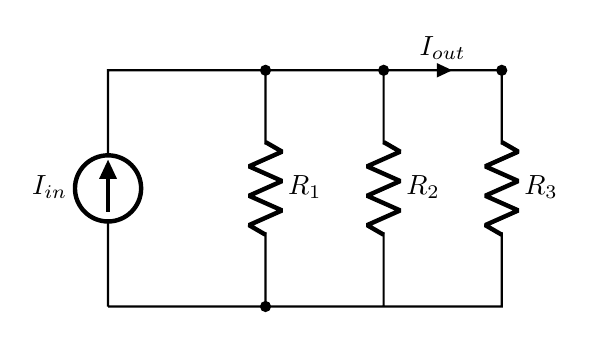
\begin{tikzpicture}[transform shape, scale=1.0,thick]
\ctikzset{bipoles/thickness=2}
\ctikzset{tubes/thickness=4}
\tikzset{anode/.style={dynode,
circuitikz/monopoles/dynode/arc angle=90},
photocatode/.style={dynode,
circuitikz/monopoles/dynode/arc pos=1,
circuitikz/monopoles/dynode/top width=0},
}
\draw (0,0) to[isource, l=$I_{in}$] (0,3)
to[short, -*] (2,3)
to[R=$R_1$] (2,0) -- (3,0)
(2,3) to[short, -*] (3.5,3)
(3.5,3) to[R=$R_2$] (3.5,0) -- (0,0)
(3.5,3) to[short, -*, i=$I_{out}$] (5,3)
to[R=$R_3$]
(5,0) to[short, -*] (2,0);

\end{tikzpicture}  
\end{document}